%%% Folie
{
\small

\begin{frame}{Ausgangslage}
    \parbox{\linewidth}{
        In seiner Standardkonfiguration ist der Raspberry Pi nur begrenzt für größere
        IoT-Anwendungsfälle geeignet, da das mitgelieferte Raspbian-Betriebssystem
        hierfür nicht ausgelegt ist. Dies liegt daran, dass der Raspberry Pi
        hauptsächlich als einfaches Lern- und Experimentiergerät in der Tradition
        früherer Heimcomputer entworfen wurde. Jedoch lässt sich das Betriebssystem
        sehr leicht anpassen oder durch ein maßgeschneidertes Embedded Linux ersetzen.
    }

    \medskip

    \begin{columns}[b,onlytextwidth]
        \column{.48\textwidth}
        \begin{center}
            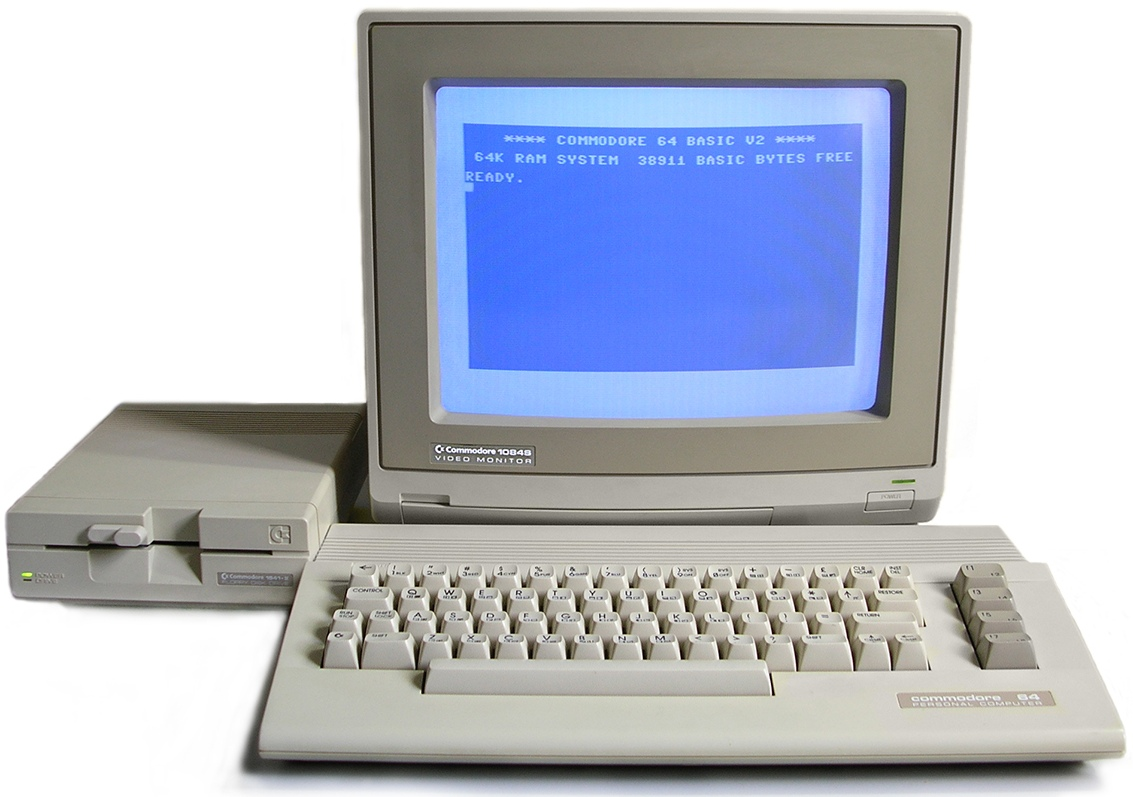
\includegraphics[width=.9\textwidth]{8-linux/img/c64}
        \end{center}
        \parbox{\linewidth}{
            \footnotesize
            \textbf{Commodore 64:}
            Beispiel für einen weit verbreiteten Heimcomputer der 1980er-Jahre
            mit eingebautem BASIC-Interpreter
        }

        \column{.48\textwidth}
        \begin{center}
            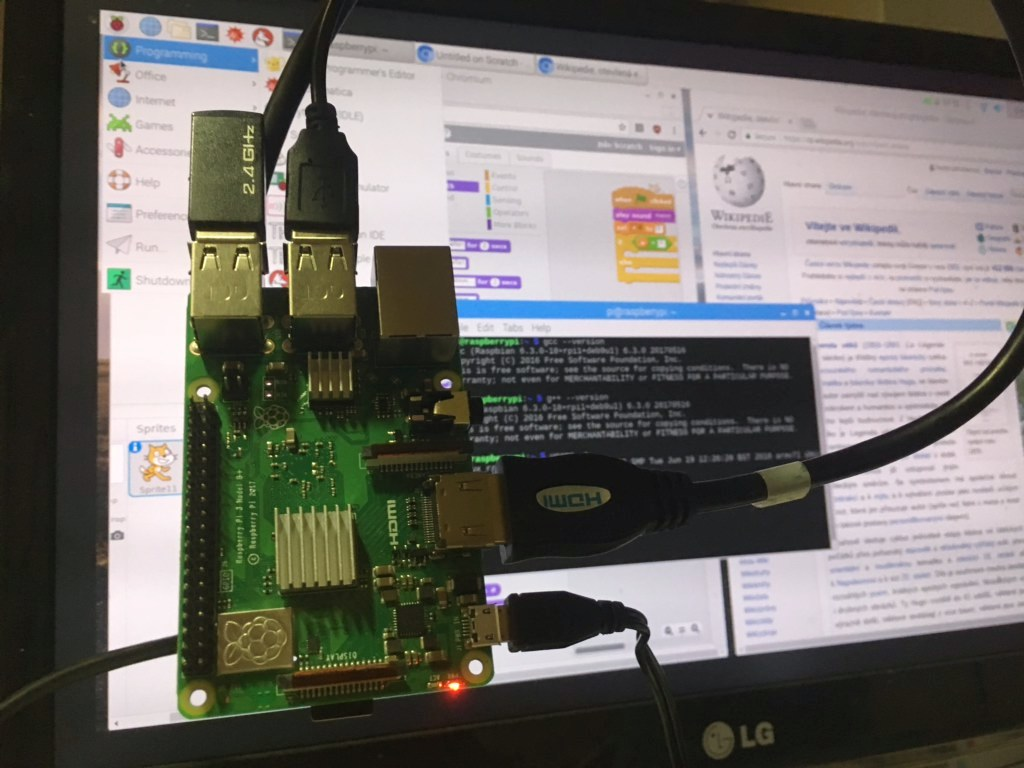
\includegraphics[width=.85\textwidth]{8-linux/img/raspi}
        \end{center}
        \parbox{\linewidth}{
            \footnotesize
            \textbf{Rasbperry Pi:} Modermer Versuch, einen Computer zum
            Experimentieren und Programmieren Lernen zu bauen
        }
    \end{columns}
\end{frame}
}

%%% Folie
\begin{frame}{Lernziele}
    \begin{block}{Bestandteile eines Linux-Systems}
        \begin{itemize}
            \item Den typischen Aufbau eines Linux-Systems beschreiben können
            \item Den Filesystem Hierarchy Standard kennen und verstehen
            \item Die Benutzer- und Rechteverwaltung von Linux nutzen können
            \item Das Partitionsschema des Raspberry Pi kennen und verstehen
            \item Den Bootvorgang des Raspberry Pi vollständig erklären können
            \item Die Aufgaben und Funktionsweise des Init-Systems erklären können
            \item Eigene Python-Programme installieren und automatisch starten
        \end{itemize}
    \end{block}

    \begin{block}{Erstellung eigener Linux-Systeme}
        \begin{itemize}
            \item Die Vorgehensweise beim Bau eigener Images kennen und verstehen
            \item Ein geeignetes Toolkit zum Bau von Linux-Systemen auswählen können
            \item Eigene Linux Images mit den vorgestellten Toolkits erzeugen können
            \item Eigene Programme in die selbst erstellten Images integrieren können
        \end{itemize}
    \end{block}
\end{frame}

%%% Folie
\begin{frame}{Inhaltsübersicht}
    \tikzset{
        MyTitle/.style={
            align=left,
            text=blue!65!purple,    % 65% blue, 35% purple
            anchor=north west,
            font=\large,
        },
        MyNode1/.style={
            below=2pt,
            align=left,
            anchor=north west,
            font=\footnotesize
        },
        MyNode2/.style={
            above=2pt,
            align=left,
            anchor=south west,
            font=\footnotesize
        },
        MyNumber/.style={
            text=white,
            font=\scriptsize
        }
    }

    % Vgl. https://tex.stackexchange.com/a/18201
    \pgfdeclarelayer{bg}
    \pgfsetlayers{bg, main}

    \begin{columns}
        \column{\dimexpr\paperwidth-1.4cm}
        \begin{tikzpicture}
            % Bestandteile eines Linux-Systems
            \node[MyTitle] at (0,0) {Bestandteile eines Linux-Systems};
            \filldraw[fill=darkred]
                ( 0,-0.6) circle(4pt) node(pi-1){} node[MyNumber]{1}  node[MyNode1]{Der grundsätzliche Aufbau \\ eines Linux-Systems}
                ( 4,-0.6) circle(4pt) node(pi-2){} node[MyNumber]{2}  node[MyNode1]{Der Linux Filesystem \\ Hierarchy Standard}
                ( 8,-0.6) circle(4pt) node(pi-3){} node[MyNumber]{3}  node[MyNode1]{Benutzer- und Rechte- \\ verwaltung unter Linux};
            \filldraw[fill=gray!50]
                (11,-0.6) circle(4pt) node(pi-tr){}
                (11,-2.6) circle(4pt) node(pi-br){};
            \filldraw[fill=darkred]
                ( 8,-2.6) circle(4pt) node(pi-4){} node[MyNumber]{4}  node[MyNode2]{Der Bootvorgang des \\ Raspberry Pi im Detail}
                ( 4,-2.6) circle(4pt) node(pi-5){} node[MyNumber]{5}  node[MyNode2]{Konfiguration des \\ Linux-Startvorgangs}
                ( 0,-2.6) circle(4pt) node(pi-6){} node[MyNumber]{6}  node[MyNode2]{Verweis auf weitere, \\ oft benötigte Konzepte};

            % Erstellung eigener Linux-Systeme
            \node[MyTitle] at (0,-3.4) {Erstellung eigener Linux-Systeme};
            \filldraw[fill=darkred]
                ( 0,-4.0) circle(4pt) node(mk-1){} node[MyNumber]{7}  node[MyNode1]{Generelles Vorgehen beim \\ Bau eines Firmware-Images}
                ( 4,-4.0) circle(4pt) node(mk-2){} node[MyNumber]{8}  node[MyNode1]{Vergleich verschiedener \\ Baukästen für Linux}
                ( 8,-4.0) circle(4pt) node(mk-3){} node[MyNumber]{9}  node[MyNode1]{Linux-Images bauen \\ mit Rasbperry Pi Gen};
            \filldraw[fill=gray!50]
                (11,-4.0) circle(4pt) node(mk-tr){}
                (11,-6.0) circle(4pt) node(mk-br){};
            \filldraw[fill=darkred]
                ( 8,-6.0) circle(4pt) node(mk-4){} node[MyNumber]{10} node[MyNode2]{Linux-Images bauen \\ mit Buildroot}
                ( 4,-6.0) circle(4pt) node(mk-5){} node[MyNumber]{11} node[MyNode2]{Linux-Images bauen \\ mit Ubuntu Core}
                ( 0,-6.0) circle(4pt) node(mk-6){} node[MyNumber]{12} node[MyNode2]{Fazit und Ausblick};

            % Verbindungslinien
            \begin{pgfonlayer}{bg}
                \draw (pi-1) -- (pi-2) -- (pi-3) -- (pi-tr) -- (pi-br) -- (pi-4) -- (pi-5) -- (pi-6);
                \draw[gray, densely dashed] (pi-6) -- (mk-1);
                \draw (mk-1) -- (mk-2) -- (mk-3) -- (mk-tr) -- (mk-br) -- (mk-4) -- (mk-5) -- (mk-6);
            \end{pgfonlayer}
        \end{tikzpicture}
    \end{columns}
\end{frame}

%-------------------------------------------------------------------------------
\section{Bestandteile eines Linux-Systems}
%-------------------------------------------------------------------------------

%%% Folie
\begin{frame}{Beispiele für Linux-basierte Betriebssysteme}
    \parbox{\linewidth}{
        \footnotesize
        Linux bezeichnet im engeren Sinne kein Betriebssystem sondern nur einen
        Kernel, der die Grundlage für viele Betriebssysteme (Linux-Distributionen)
        auf den unterschiedlichsten Computersystemen bildet. Linux kann dabei auf
        nahezu jeder Hardware betrieben werden.
        \medskip
    }

    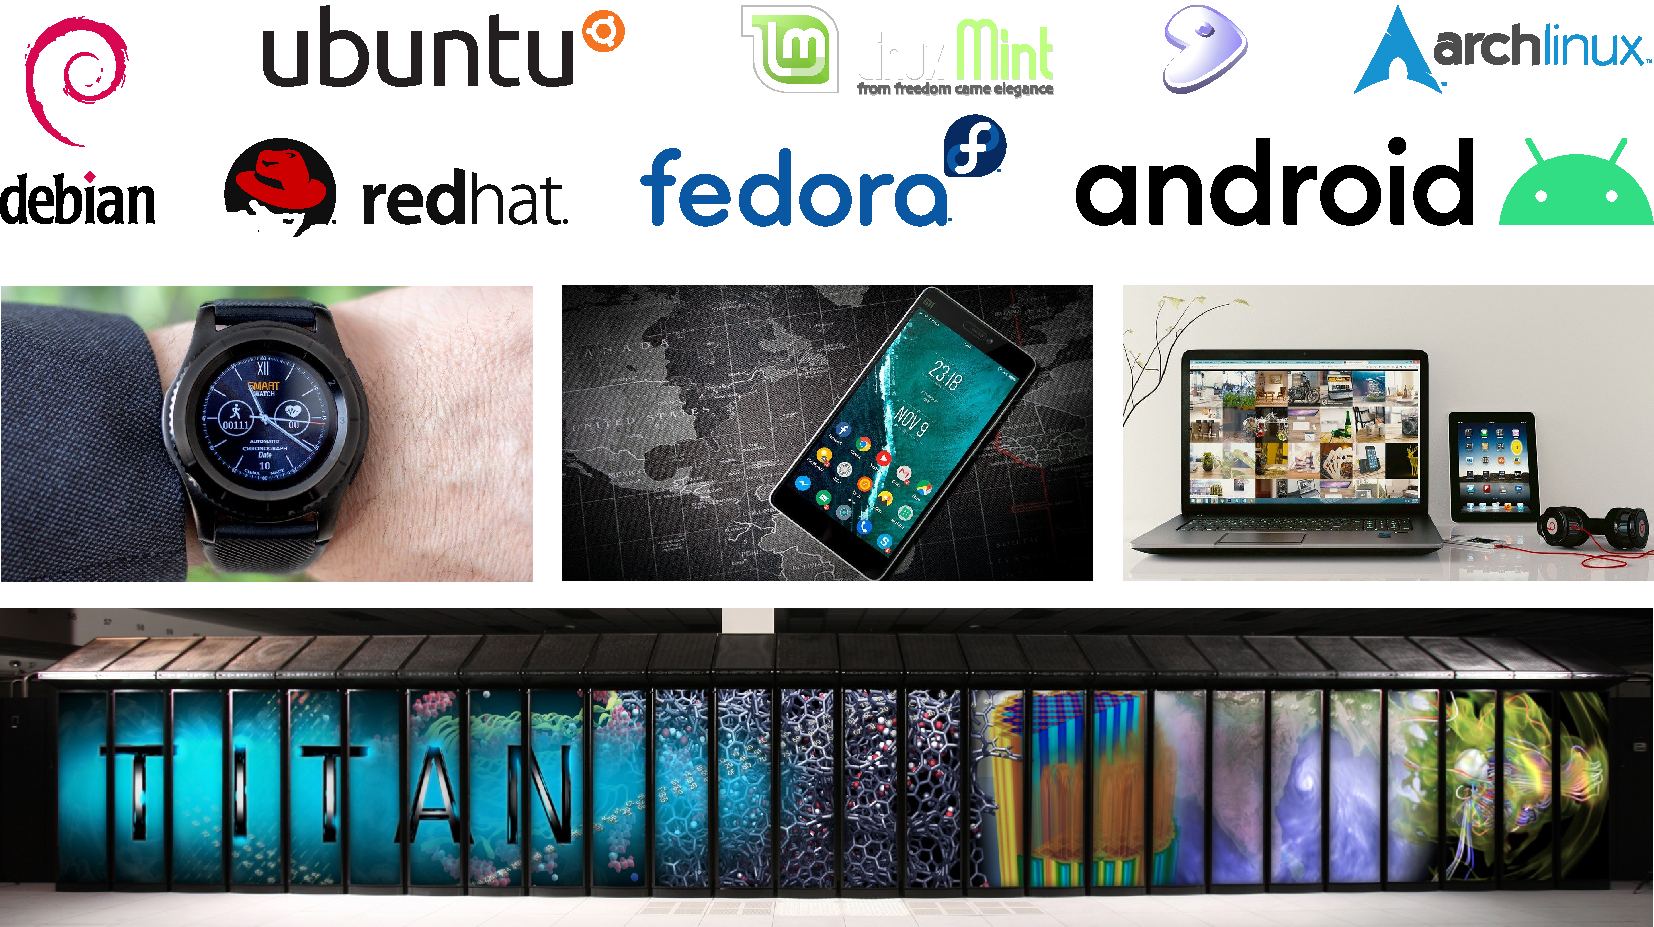
\includegraphics[width=\textwidth]{8-linux/img/linux-beispiele}
\end{frame}

%%% Folie
{
\footnotesize
\setlength{\leftmargini}{1.2em}

\begin{frame}{Kernel vs. Userland}
    \parbox{\linewidth}{
        Linux-basierte Betriebssysteme setzen sich immer aus dem \textbf{Kernel}
        und dem \textbf{Userland} zusammen. Der Kernel beinhaltet dabei lediglich
        die Grundfunktionen für Hardwarezugriffe, Multitasking, Speicherverwaltung
        usw. Alle anderen Teile des Betriebssystems sind Bestandteil des Userlands
        und können somit stark variieren.
    }

    \vfill

    {
        \scriptsize

        \begin{columns}[T,onlytextwidth]
            \column{.49\textwidth}
            \begin{itemize}
                \justifying

                \item \textbf{Bibliotheken:} Von den installierten Programmen
                benötigte Quellcode-Bibliotheken mit gemeinsamen Funktionen.
                Zum Beispiel \texttt{libc} oder \texttt{libgtk}.

                \item \textbf{Systemdienste:} Hintergrundjobs und Hilfsprogramme des
                Betriebssystems. Zum Beispiel NTP-Daemon, Druckerspooler oder die
                Shell bzw. grafische Desktopumgebung.

                \item \textbf{Anwendungen:} Nicht direkt zum Betriebssystem gehörende,
                jedoch zur Nutzung durch die Anwender*innen vorgesehene Programme, wie
                zum Beispiel Webbrowser oder Media Player.
            \end{itemize}

            \column{.49\textwidth}
            \begin{itemize}
                \justifying

                \item \textbf{Variable Daten:} Während dem regulären Systembetrieb
                anfallende Verwaltungsdaten, wie Systemprotokolle, temporäre Dateien
                oder zwischengespeicherte Druckaufträge.

                \item \textbf{Benutzerdaten:} In der Hoheit der Benutzer*innen liegende
                Dateien, wie zum Beispiel Bilder oder Dokumente.
            \end{itemize}
        \end{columns}
    }

    \vfill
    $\Rightarrow$ \textbf{GNU/Linux:} Linux-Kernel mit GNU-Userland (plus weiteren Bestandteilen) \\
    $\Rightarrow$ \textbf{Android:} Linux-Kernel mit nahezu komplett in Java entwickeltem Userland

    \vfill
    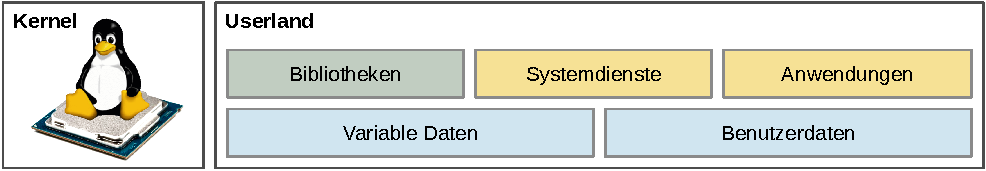
\includegraphics[width=\textwidth]{8-linux/img/linux-bestandteile}
\end{frame}
}

%%% Folie
{
\footnotesize

\begin{frame}[allowframebreaks]{Der Linux Filesystem Hierarchy Standard}
    \begin{center}
        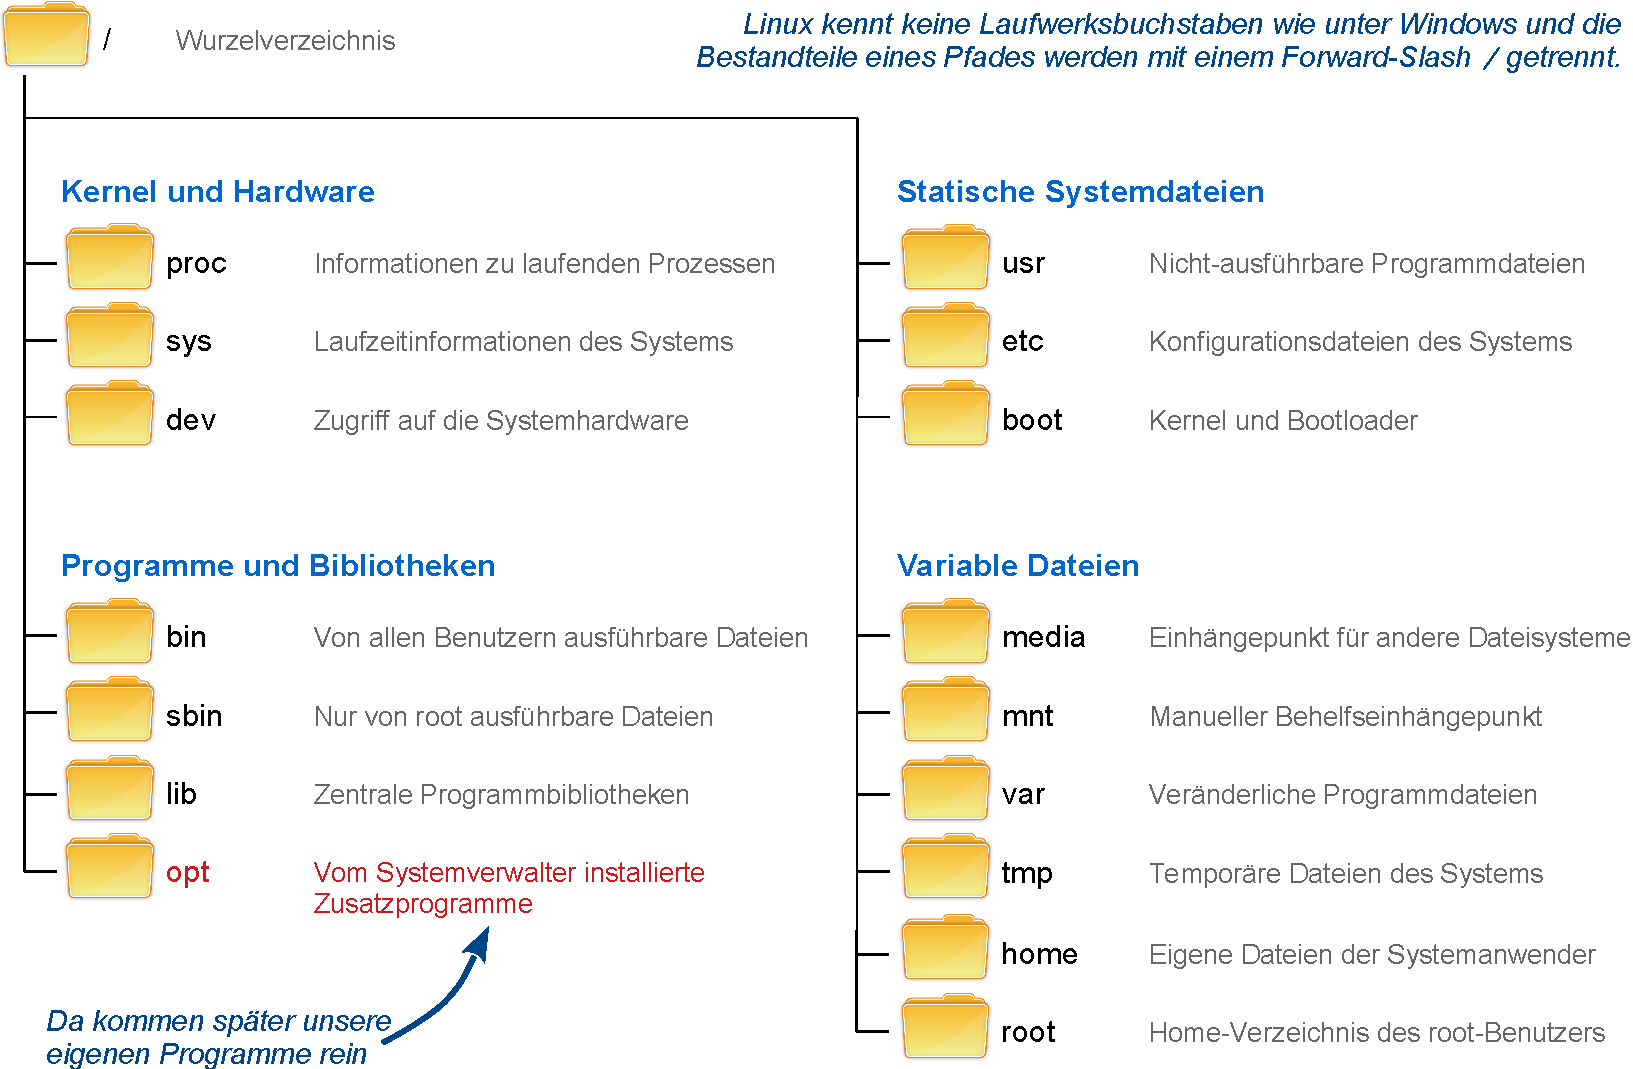
\includegraphics[width=\textwidth]{8-linux/img/fhs-verzeichnisse}
    \end{center}

    \framebreak

    \begin{columns}[T]
        \column{.8\textwidth}
        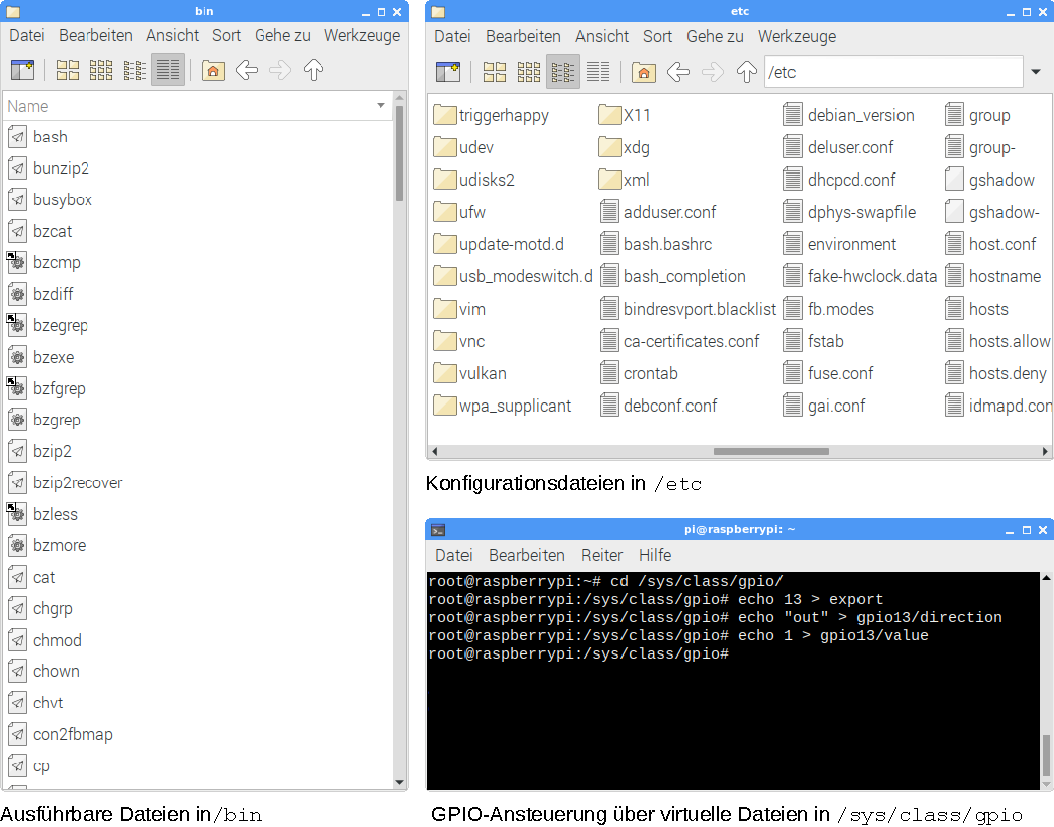
\includegraphics[width=\textwidth]{8-linux/img/fhs-beispiele}

        \column{.3\textwidth}
        \parbox{\linewidth}{
            Aufgrund der konzeptionellen Nähe zu Unix ist unter Linux fast alles
            eine Datei. Die Konfiguration des Systems erfolgt deshalb genau so
            durch Editieren von Konfigurationsdateien, wie der Zugriff auf einen
            Hardwarebaustein nicht viel mehr als das Lesen und Schreiben virtueller
            Dateien erfordert.
        }
    \end{columns}
\end{frame}
}

%%% Folie
{
\footnotesize

\begin{frame}[allowframebreaks]{Benutzer- und Rechteverwaltung unter Linux}
    \begin{columns}[onlytextwidth]
        \column{.55\textwidth}
        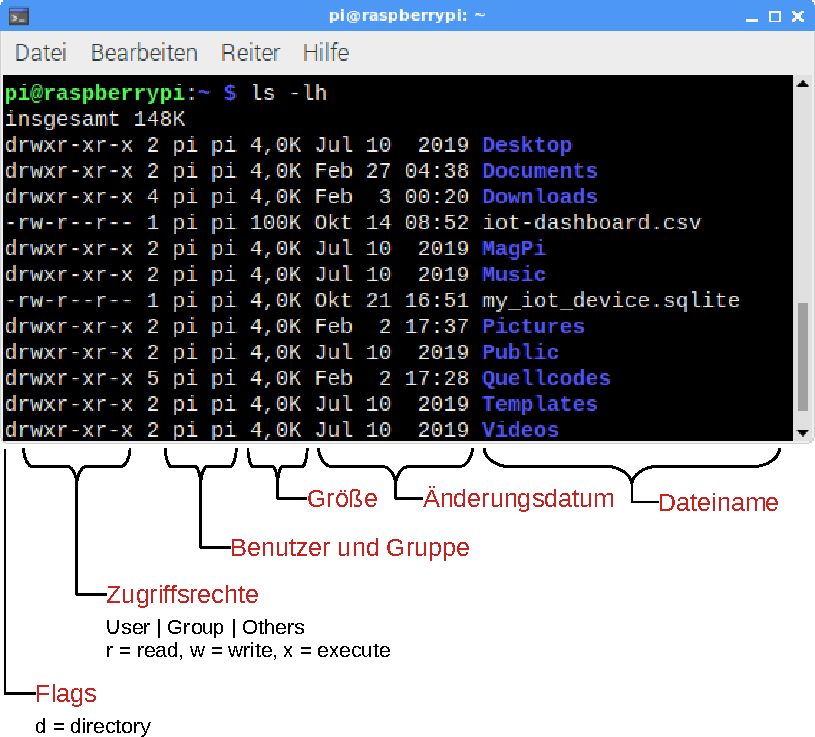
\includegraphics[width=\textwidth]{8-linux/img/rechte-dateizugriff}

        \column{.4\textwidth}
        \parbox{\linewidth}{
            Alle Einträge im Dateisystem sind immer genau einem Benutzerkonto
            und einer Benutzergruppe zugeordnet. Zusätzlich besitzen sie ein
            Bit-Feld mit Zugriffsrechten für

            \begin{itemize}
                \item den Benutzer,
                \item die Benutzergruppe,
                \item den Rest der Welt.
            \end{itemize}

            Über dieses Feld wird gesteuert, ob Lese-, Schreib- oder ausführende
            Zugriffe erlaubt sind.

            \medskip

            \glqq{}Ausführen\grqq{} bedeutet bei einer Datei, diese als Programm
            zu starten. Bei einem Verzeichnis bedeutet es, die Inhalte des
            Verzeichnisses zu sehen.

            \medskip

            Die Berechtigungsprüfung wird immer mit dem Benutzerkonto durchgeführt,
            unter dessen Namen ein zugreifendes Programm läuft.
        }
    \end{columns}

    \medskip
    \textbf{Wichtige Befehle}

    \begin{columns}[onlytextwidth]
        \column{.33\textwidth}
        \texttt{chown} \\ Benutzer/Gruppe ändern

        \column{.33\textwidth}
        \texttt{chmod} \\ Zugriffsrechte ändern

        \column{.33\textwidth}
        \texttt{sudo} \\ Programm unter anderem Benutzer starten
    \end{columns}

    %%
    \framebreak

    \begin{center}
        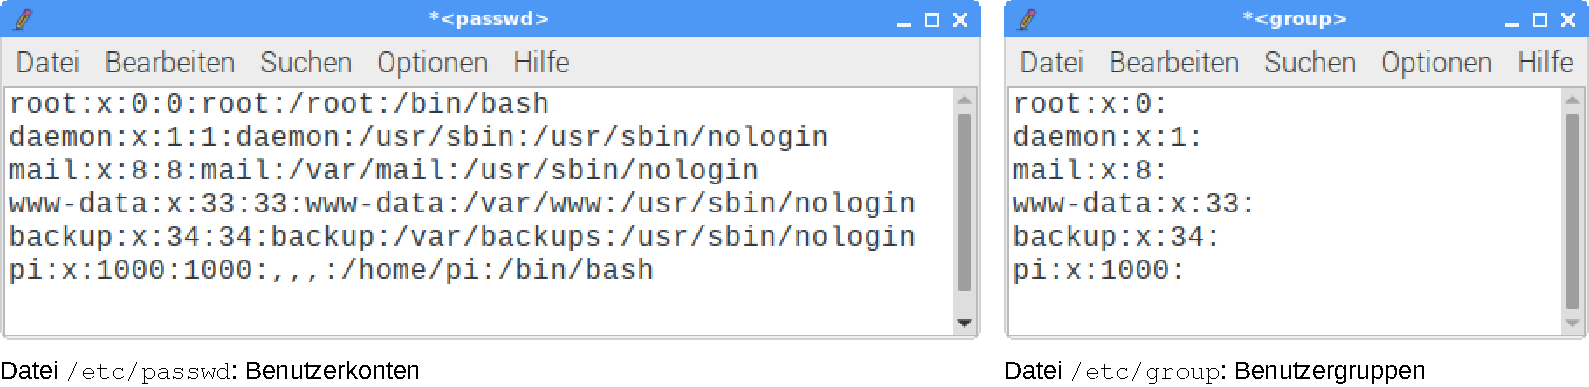
\includegraphics[width=\textwidth]{8-linux/img/rechte-konfiguration}
    \end{center}

    \parbox{\linewidth}{
        Die Benutzerkonten und Benutzergruppen sind in den Dateien
        \texttt{/etc/passwd} und \texttt{/etc/group} definiert. Jeder
        Benutzer bzw. jede Benutzergruppe bekommt hier eine numerische ID
        zugewiesen, die sehr oft nach folgendem Schema vergeben wird:
    }

    \medskip

    {
        \scriptsize
        \renewcommand{\arraystretch}{1.4}
        \setlength{\tabcolsep}{0em}

        \begin{tabularx}{\textwidth}{p{.11\textwidth} p{.2\textwidth} X}
            \hline
            \textbf{UID/GID} & \textbf{Bezeichnung} & \textbf{Bedeutung} \\
            \hline

            0 & Benutzer \texttt{root} & Superuser mit maximalen Berechtigungen \\
            1 -- 999 & Systembenutzer & Technische Benutzer zur Ausführung der Systemdienste \\
            $\geq$ 1000 & Interaktive Benutzer & Menschliche Benutzer mit Login-Möglichkeit \\
            \hline
        \end{tabularx}
    }

    \medskip
    \textbf{Wichtige Befehle}
    {
        \setlength{\leftmargini}{1.2em}
        \begin{columns}[T, onlytextwidth]
            \column{.5\textwidth}
            \begin{itemize}
                \item \texttt{adduser}: Neues Benutzerkonto anlegen
                \item \texttt{deluser}: Benutzerkonto löschen
                \item \texttt{usermod}: Benutzerkonte bearbeiten
            \end{itemize}

            \column{.5\textwidth}
            \begin{itemize}
                \item \texttt{passwd}: Benutzerpasswort ändern
                \item \texttt{groupadd}: Neue Benutzergruppe anlegen
                \item \texttt{delgroup}: Benutzergruppe löschen
            \end{itemize}
        \end{columns}
    }
\end{frame}
}

% Partitionsschema das Pi (Hinweis auf weitere Partitionen und /etc/fstab)
% Bootvorgang Pi, pstree
% PID 1. Beispiele
% Fallbeispiel: Eigenes Skript starten

% Ausblick: Weitere Linux-Konzepte


%%%% Folie
%{
%\footnotesize

%\begin{frame}[allowframebreaks]{Typischer Aufbau eines Linux-Systems}
    %\begin{columns}
        %\column{.45\textwidth}
        %\begin{center}
            %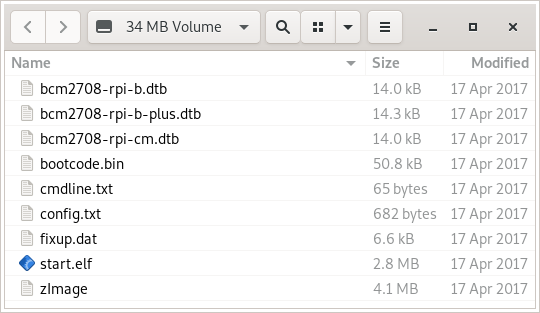
\includegraphics[width=\textwidth]{8-linux/img/partition-boot}
            %\smallskip
            %Bootpartition des Raspberry Pi
        %\end{center}

        %\column{.45\textwidth}
        %\begin{center}
            %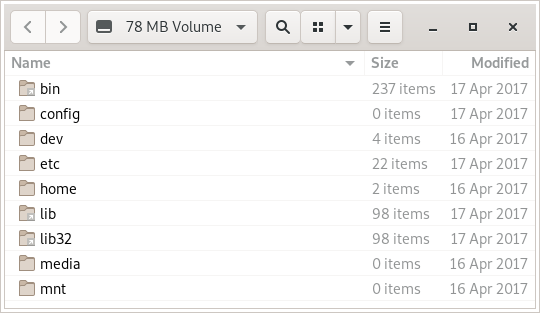
\includegraphics[width=\textwidth]{8-linux/img/partition-system}
            %\smallskip
            %Systempartition des Raspberry Pi
        %\end{center}
    %\end{columns}

    %\framebreak
    %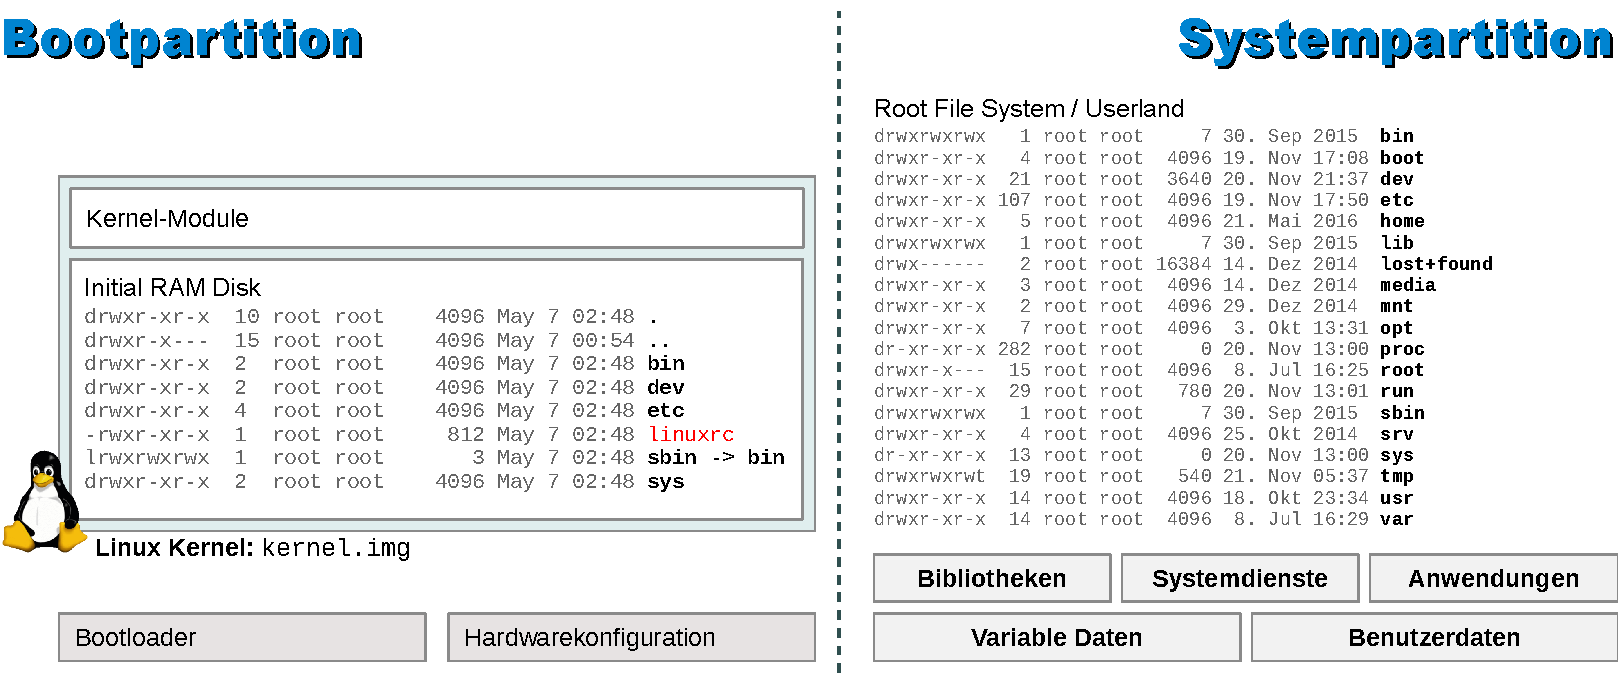
\includegraphics[width=\textwidth]{8-linux/img/linux-aufbau}
    %\smallskip

    %\parbox{\linewidth}{
        %Linux-basierte Betriebssysteme setzen sich immer aus einem \textbf{Kernel}
        %und dem \textbf{Userland} zusammen. Wie für eingebettete Systeme typisch,
        %befinden sich beide beim Raspberry Pi in getrennten Partitionen, wobei die
        %Boot-Partition zusätzlich noch den Bootloader und Konfigurationsdateien zur
        %Initialisierung der Hardware beinhaltet.
    %}

    %{
        %\bigskip
        %\scriptsize

        %\begin{columns}[T, onlytextwidth]
            %\column{.49\textwidth}
            %\parbox{\linewidth}{
                %\textbf{Systemdienste:} Systemnahe Programme, Hintergrundjobs und
                %Serverprogramme
            %}

            %\column{.49\textwidth}
            %\parbox{\linewidth}{
                %\textbf{Anwendungen:} Zusätzliche Anwendungsprogramme, die keine
                %Systemfunktionen im engeren Sinne erfüllen
            %}
        %\end{columns}

        %\medskip

        %\begin{columns}[T, onlytextwidth]
            %\column{.49\textwidth}
            %\parbox{\linewidth}{
                %\textbf{Variable Daten:} Während der Benutzung des Systems automatisch
                %anfallende Daten
            %}

            %\column{.49\textwidth}
            %\parbox{\linewidth}{
                %\textbf{Benutzerdaten:} Durch den Endanwender erzeugte und verwaltete
                %Daten
            %}
        %\end{columns}
    %}

    %\framebreak
    %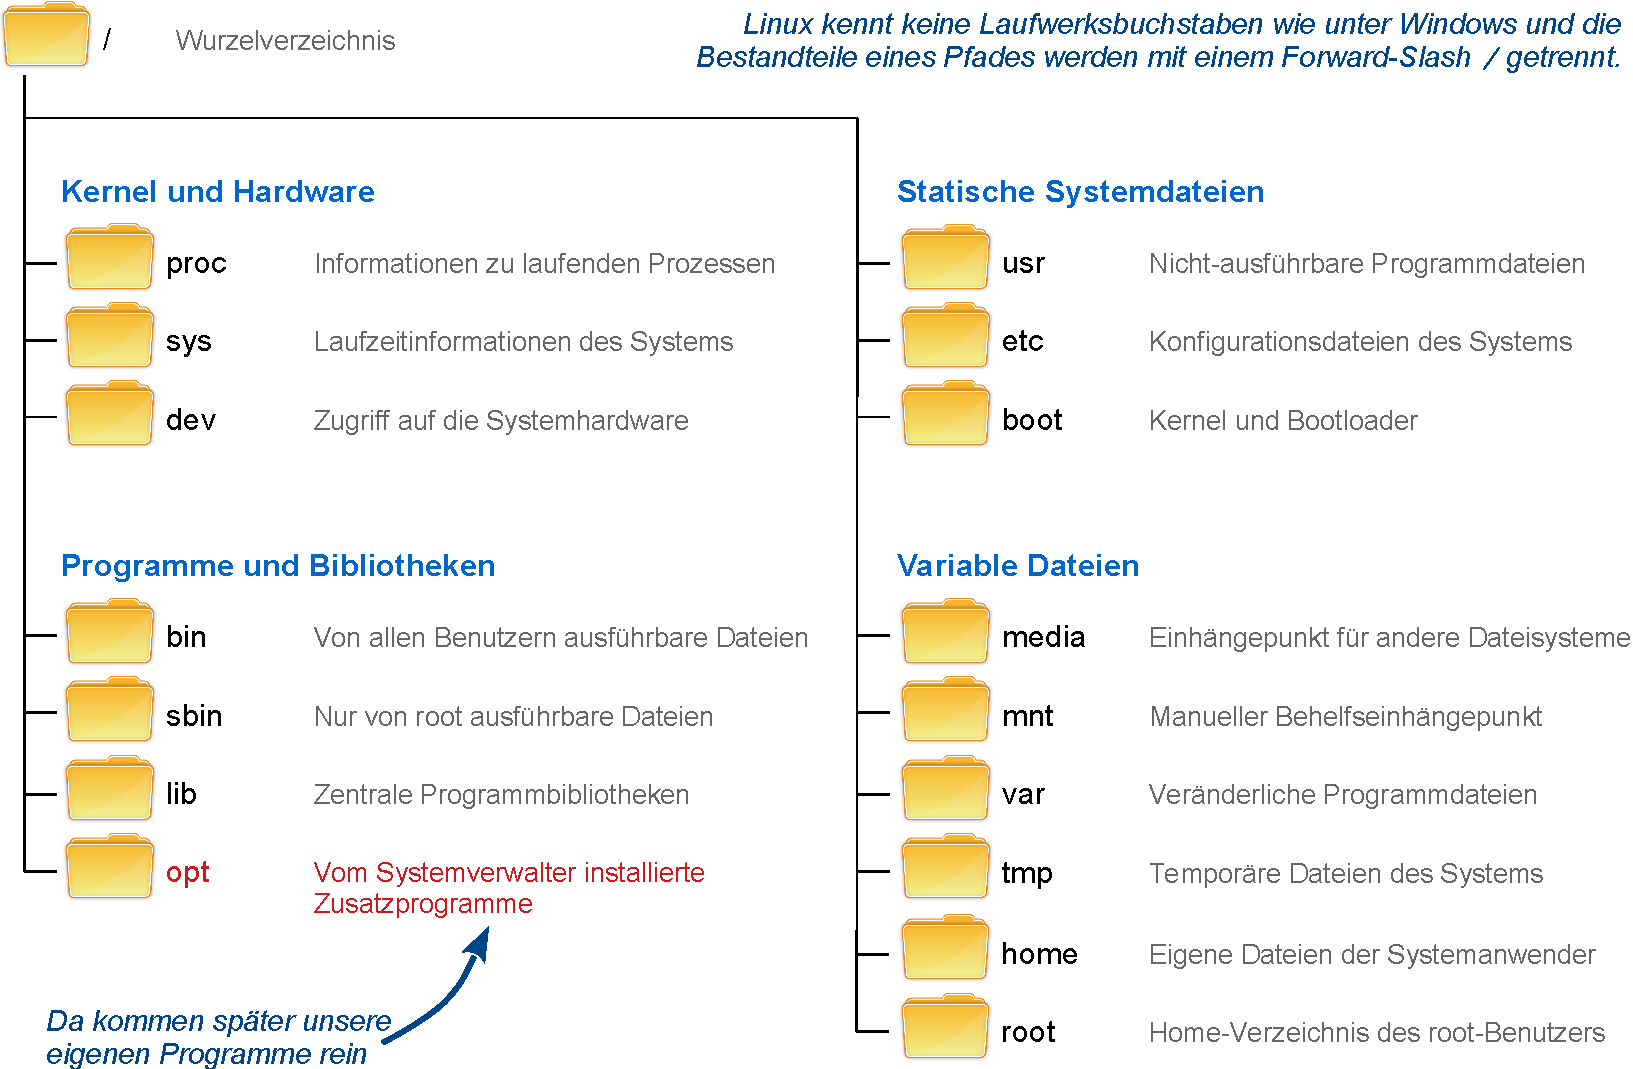
\includegraphics[width=\textwidth]{8-linux/img/fhs-verzeichnisse}
%\end{frame}
%}

%%% Folie
\begin{frame}{Der Bootvorgang des Raspberry Pi im Detail}
    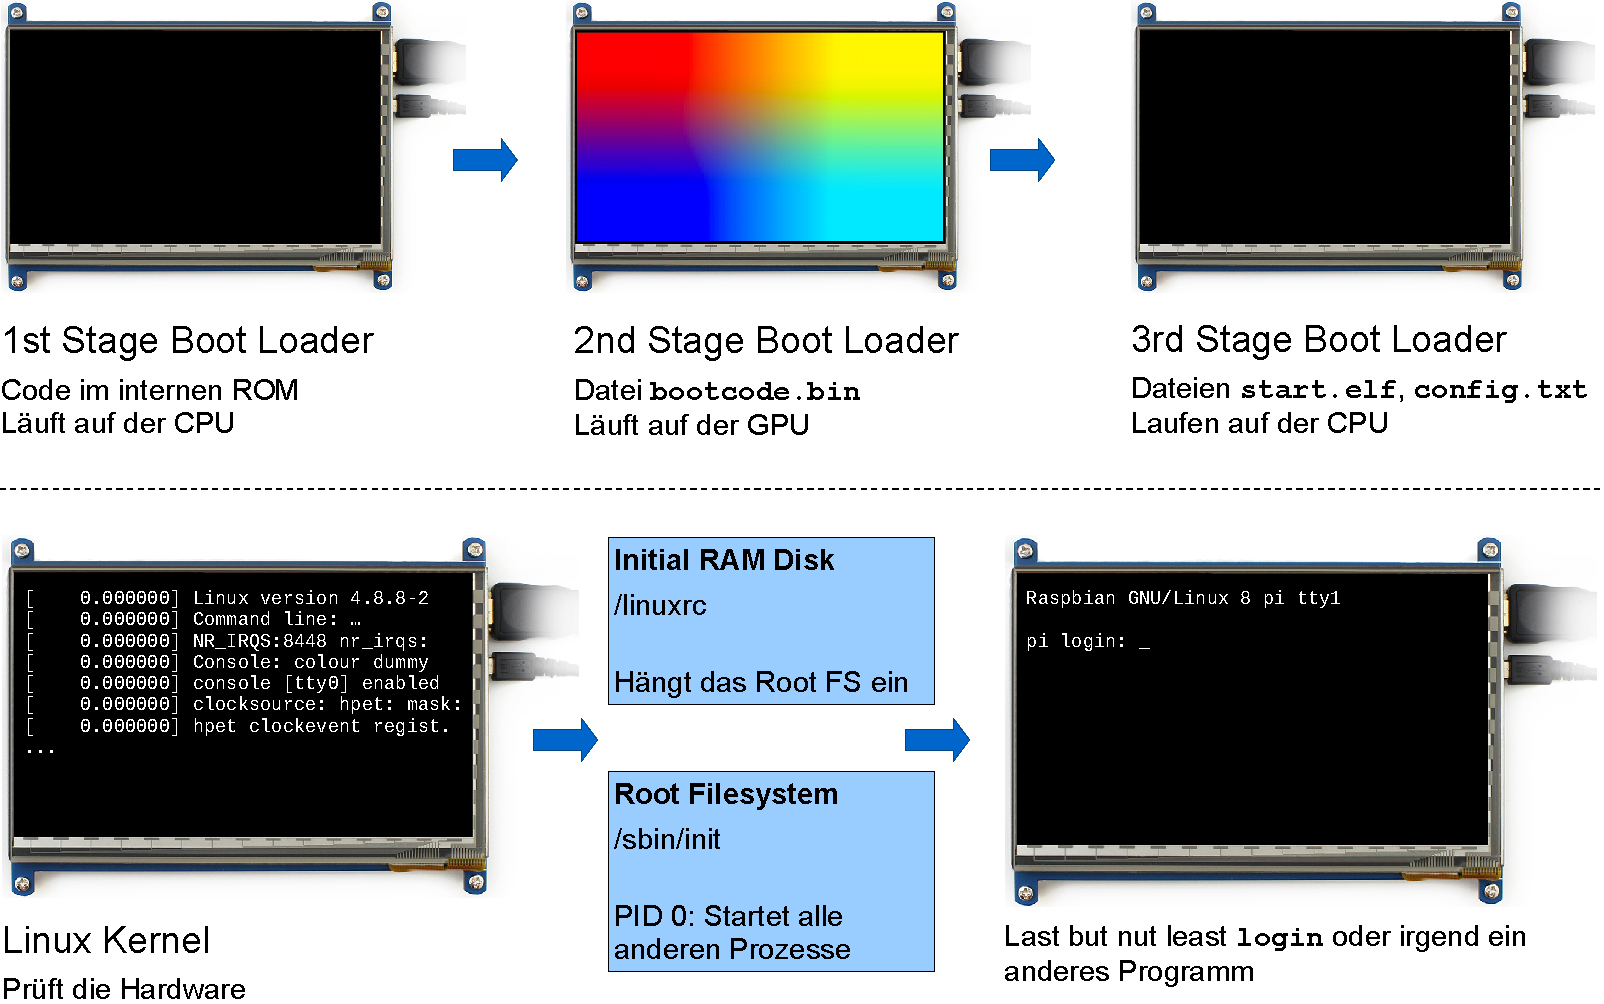
\includegraphics[width=\textwidth]{8-linux/img/pi-bootvorgang}
\end{frame}


%-------------------------------------------------------------------------------
\section{Erstellung eigener Linux-Systeme}
%-------------------------------------------------------------------------------

%%% Folie
\begin{frame}{Generelles Vorgehen beim Bau eines Firmware-Images}
    TODO
\end{frame}

%%% Folie
\begin{frame}{Vergleich verschiedener Baukästen für Linux}
    TODO
\end{frame}

%%% Folie
\begin{frame}{Linux-Images bauen mit Raspberry Pi Gen}
    TODO
\end{frame}

%%% Folie
\begin{frame}{Linux-Images bauen mit Buildroot}
    TODO
\end{frame}

%%% Folie
\begin{frame}{Linux-Images bauen mit Ubuntu Core}
    TODO
\end{frame}

%%% Folie
\begin{frame}{Fazit und Ausblick}
    TODO
\end{frame}

